\section{Struttura dell'UP}
\label{concept:UP-structure}
Lo Unified Process è strutturato a \textbf{fasi}. Una fase comprende più iterazioni. In ogni fase sono prioritirizzate alcune attività rispetto ad altre. Alla fine di ogni iterazione viene generata una {baseline}, questa viene valutata secondo alcune precise condizioni che, se verificate, dichiarano conclusa la fase. La {baseline} che verifica queste condizioni viene detta \textbf{milestone}. Le fasi del Processo Unificato sono \textbf{quattro}: \hyperref[concept:avvio]{avvio}, \hyperref[concept:elaborazione]{elaborazione}, \hyperref[concept:costruzione]{costruzione} e \hyperref[concept:transizione]{transizione}.
\begin{figure}[h]
    \centering
    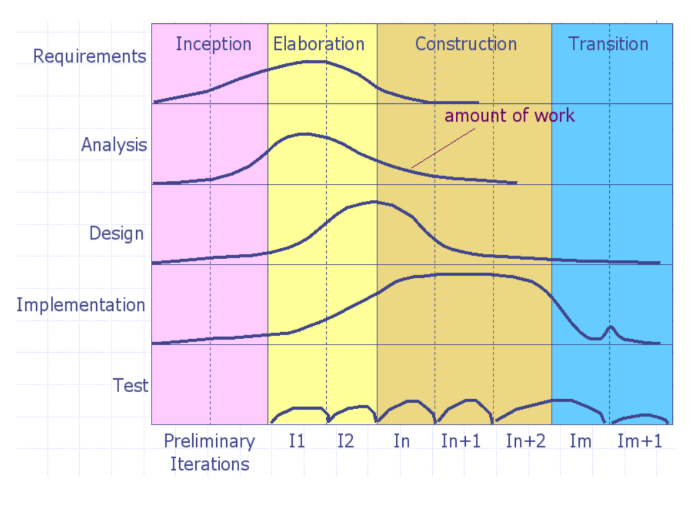
\includegraphics[width=0.75\linewidth]{IDSTEORIA//Immagini/ProcessoUnificato/UPStructure.png}
    \caption{Distribuzione delle varie attività nelle fasi dell'UP}
    \label{fig:UPStructure}
\end{figure}
\subsection{Avvio (o Inception)}
\label{concept:avvio}
\paragraph{Attività Principali} Identificazione degli {stakeholder}, raccolta dei requisiti ad alto livello, definizione di uno Use Case Diagram iniziale, stima dei costi, analisi di fattibilità, valutazione dei rischi, definizione di un piano di progetto.
\paragraph{Obiettivi} Definire ambito del sistema, identificare principali casi d'uso, valutare la fattibilità del progetto, stabilire un business case solido.
\paragraph{Milestone}
\begin{itemize}
    \item UC Diagram contenente 10-20\% dei Casi D'Uso ben definiti
    \item Go-no go: decisione se il progetto è fattibile e vale la pena continuare
    \item Business case
    \item Vision document
    \item Lista ed analisi dei rischi
\end{itemize}
\subsection{Elaborazione (o Elaboration)}
\label{concept:elaborazione}
\paragraph{Attività Principali} Sviluppo dell'architettura software, completamento di use case significativi, definizione dell'architettura del sistema, inizio della documentazione tecnica, valutazione di rischi tecnici tramite prototipi. ù
\paragraph{Obiettivi} Definire e validare architettura software, affinare i requisiti, ridurre i rischi più significativi, produrre un piano di progetto dettagliato per le fasi successive.
\paragraph{Milestone}
\begin{itemize}
    \item UC Diagram contenente 80-90\% dei Casi D'Uso ben definiti
    \item Architettura stabile ed \textbf{eseguibile}
    \item Piano di progetto revisionato
    \item Stima dei rischi revisionata
    \item Accordo finale tra le parti firmato
\end{itemize}
\subsection{Costruzione (o Construction)}
\label{concept:costruzione}
\paragraph{Attività Principali} Sviluppo iterativo del software completo, implementazione completa dei casi d'uso, scrittura, ottimizzazione, testing e documentazione del codice, gestione di eventuali cambiamenti nei requisiti, rivalutare i rischi.
\paragraph{Obiettivi} Completare l'identificazione, la descrizione e l'implementazione dei Casi D'Uso, mantenere l'integrità dell'architettura del sistema. 
\paragraph{Milestone}
\begin{itemize}
    \item Software stabile e di qualità sufficiente da essere rilasciato
    \item Verifica dei costi rispetto alla pianificazione iniziale
    \item Eventuali manuali o piani di distribuzione definiti nell'accordo tra le parti
\end{itemize}
\subsection{Transizione (o Transition)}
\label{concept:transizione}
\paragraph{Attività Principali} Testing lato utente, modifiche del design in caso siano emersi errori in fase di testing, supporto tecnico e documentazione, raccolta di feedback degli utenti, refactoring o ottimizzazione finale.
\paragraph{Obiettivi} Rilascio prodotto agli utenti finali, correzione errori, addestramento e supporto agli utenti per l'utilizzo del software.
\paragraph{Milestone}
\begin{itemize}
    \item Prodotto software ultimato e testato
    \item Uso attivo del prodotto
    \item Definizione delle strategie di supporto (es. manuale utente)
    \item Piano di Manutenzione
\end{itemize}
